\section{Transaction and recovery manager}

\begin{figure}[h!]
		\centering
		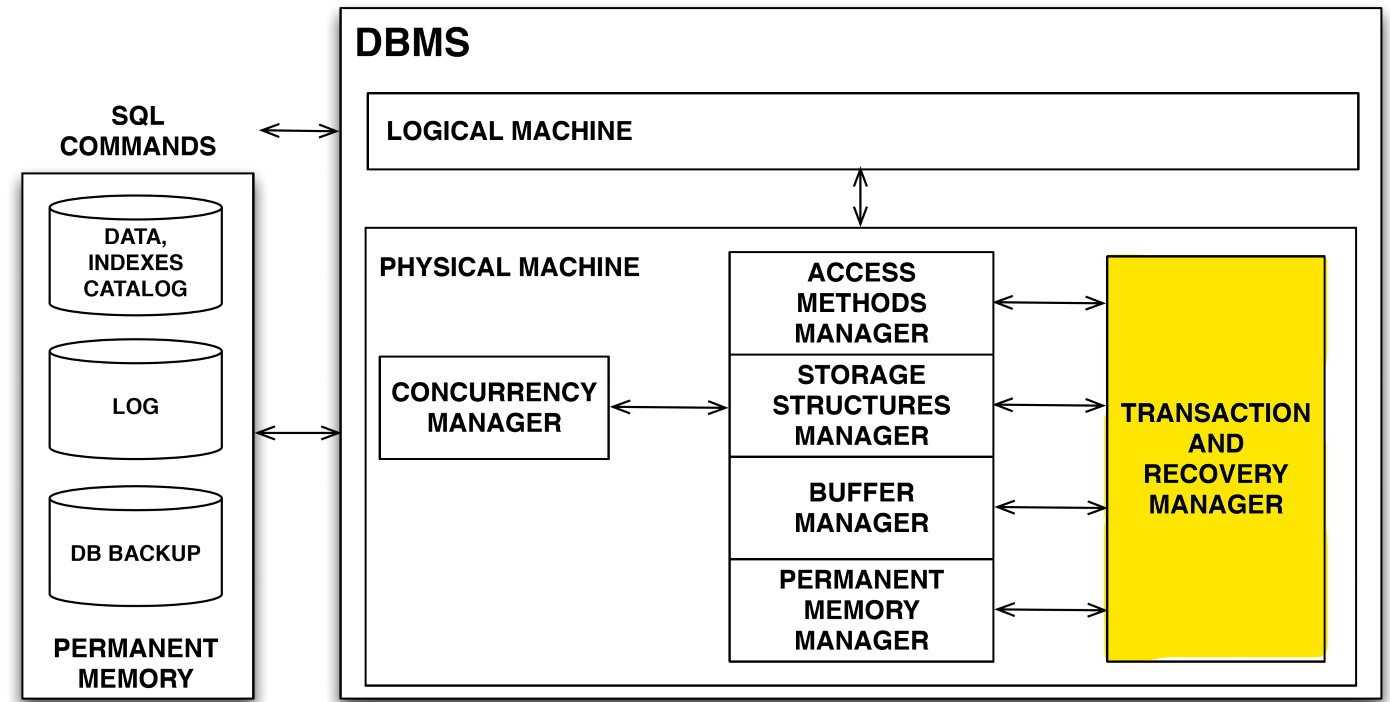
\includegraphics[scale = 0.7]{img/tr1.jpg}
		\label{tr1}
\end{figure}

One of the most important features of a DBMS are the techniques provided for the solution of the \textit{recovery} and \textit{} problems, to allow the users to assume that each of their applications is executed both as if there were no failures, and that there were no interferences with other applications running concurrently. The solutions of these problems are based on the abstraction mechanism called \textit{transaction}. The correct implementation of transactions requires some of the most sophisticated algorithms and data structures of a DBMS. In this chapter we will focus on transactions as a mechanism to protect data from failures, while in the next one we will examine the aspects of transactions concerning the concurrency control to avoid interference.

\subsection{Transactions}
A database is said to be in a \textit{consistent state} if all the integrity constraints are satisfied, and a \textit{transaction} is a mechanism to properly group operations on the database into atomic units of work. A transaction is \textit{correct} if it causes the DB to change from a consistent state to another consistent state, even in a system failure and by handling concurrent transactions.

\subsubsection{Transactions from the programmer's point of view}

\begin{tcolorbox}
A \textbf{transaction} is a sequence of operations on the DB with the following ACID properties:

\begin{itemize}
    \item \textbf{atomicity}: only transactions terminated normally (\textit{committed transactions}) change the database, otherwise the database remains unchanged;

    \item \textbf{isolation}: when a transaction is executed concurrently with others, the final effect must be the same as if it was executed alone;
    
    \item \textbf{durability} the effects of committed transactions on the DB survive system and media failures.
    
\end{itemize}

\end{tcolorbox}

\textbf{NOTE}: 

\begin{itemize}
    \item atomicity, isolation and durability are provided by a DBMS, while consistency cannot be ensured by the system when the integrity constraints are not declared;
    
    \item the isolation property is sometime called the \textit{serializability} property: when a transaction is executed concurrently with others, the final effect must be the same as a serial execution of committed transactions, i.e. the DBMS behaves as if it executes the transactions one at a time;

    \item the \textit{Transaction and Recovery Manager} guarantees the atomicity and durability properties, while the isolation property is guaranteed by the \textit{Concurrency Manager}
    
\end{itemize}


\subsubsection{Transactions from the DBMS's point of view}

\begin{tcolorbox}
A \textbf{transaction} for the DBMS is a sequence of read and write operations which start and end with the following transaction operations: 

\begin{itemize}
    \item \textit{beginTransaction}: beginning of the transaction;
    \item \textit{commit}: successful termination of the transaction and the system has to make its updates durable;
    \item \textit{abort}: abnormal termination, the system has to undo its updates.
\end{itemize}

\end{tcolorbox}

\textbf{NOTE}: the execution of the \textit{} operation does not guarantee the successful termination of the transaction, because it is possible that the transaction updates cannot be written to the permanent memory, and therefore it will be aborted.

Picture \ref{tr2} shows the different states of a transaction execution.

\begin{figure}[h!]
		\centering
		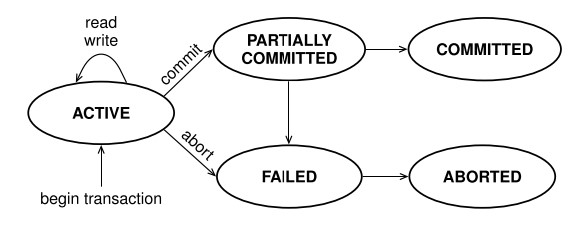
\includegraphics[scale = 1.3]{img/tr2.jpg}
		\label{tr2}
\end{figure}

\begin{itemize}

    \item a transaction enters into the \textit{active} state immediately after it starts execution, where it stays while it is executing;
    
    \item a transaction moves to the \textit{partially committed} state when it ends;
    
    \item a transaction moves to the \textit{committed} state if it has been processed successfully and all its updates on the database have been made durable. In this state we have the warranty that durability is guaranteed;    
    
    \item a transaction moves to the \textit{failed} state if it cannot be committed or it has been interrupted after a transaction failure while in the active state;
    
    \item a transaction moves to the \textit{aborted} state if it has been interrupted and all its updates on the database have been undone. In this state we have the warranty that atomicity is granted.
    
\end{itemize}

Note that the read/write and commit operations are executed by the system when required by the transaction, while the abort operation is executed by the system either when required by the transaction or when a system failure occurs, independently from the transaction requests.

\subsection{Types of failures}
We assume that the occurrence of a failure is always detected, and this causes:

\begin{itemize}
    \item the immediate interruption of a transaction or of the whole system;
    \item the execution of specific \textit{recovery procedures} to ensure that the DB only contains the updates produced by committed operations.
\end{itemize}

The following failures may occur:

\begin{itemize}

    \item \textbf{transaction failures}: is an interruption of a transaction which preserves both the buffer and the permanent memory. It may occur either due to system errors or due to error in a constraint;
    
    \item \textbf{system failure}: is a system interruption, where the content of the buffer is lost, but content of the permanent memory remains intact. In this case the DBMS is restarted;
    
    \item \textbf{media failure}: is an interruption of the DBMS in which the content of the permanent memory is corrupted or lost. In this case the recovery manager uses a backup to restore the DB.
    
\end{itemize}

\subsection{Database system model}
Looking at \ref{tr1} we notice that the permanent memory consists of three main components: the DB, the Log and the DB backup, which are used by the recovery procedure in the case of failures. Note that these three components are stored in distinct physical devices.

The \textit{Transaction and Recovery Manager} performs the following tasks:

\begin{itemize}

    \item execution of read, write, commit and abort operation on behalf of transactions and by cooperating with the \textit{Permanent Memory Manager}, the \textit{Buffer Manager} etc..;

    \item management of the log;

    \item execution of a \textit{restart} command after a system failure, in order to guarantee that the DB only contains the updates of the committed transactions;

    \item execution of techniques to prevent data loss.
    
\end{itemize}

In the next sections the data structures and algorithms used by the recovery manager will be discussed. To simplify the presentation we assume that:

\begin{enumerate}

    \item the database is just a set of pages;
    
    \item each update operation affects a single page, and it is performed by modifying an in-memory copy of the page and then by writing it to disk only when the \textit{Buffer Manager} decide to do it;
    
    \item the operation of transferring a page from the buffer to the permanent memory is an atomic operation;
    
    \item if different transactions are concurrently in execution, they read and write different pages. 
    
\end{enumerate}

\subsection{Data protection}
We saw that there exists different types of failures, but the different techniques that are used in these situations share the common principle of \textbf{redundancy}: to protect the database, the DBMS maintains some redundant information during normal execution of transactions in order to better reconstruct a consistent state, a process called \textbf{recovery}.

\subsubsection{DB backup}
The DBMS provides facilities for periodically making a backup copy of the DB.

\subsubsection{Log}
During the normal use, the history of the operations performed on the database from the last backup is stored in the \textbf{log}. 

\begin{itemize}
    \item for each transaction we write in the log when the transaction starts, commits, aborts and modifies a page;
    \item each log record is identified through the so called \textbf{LSN} (Log Sequence Number), that is assigned in a strictly increasing order. It can be viewed as the serial number of the position of the first character of the record in the file;
\end{itemize}

\begin{figure}[h!]
		\centering
		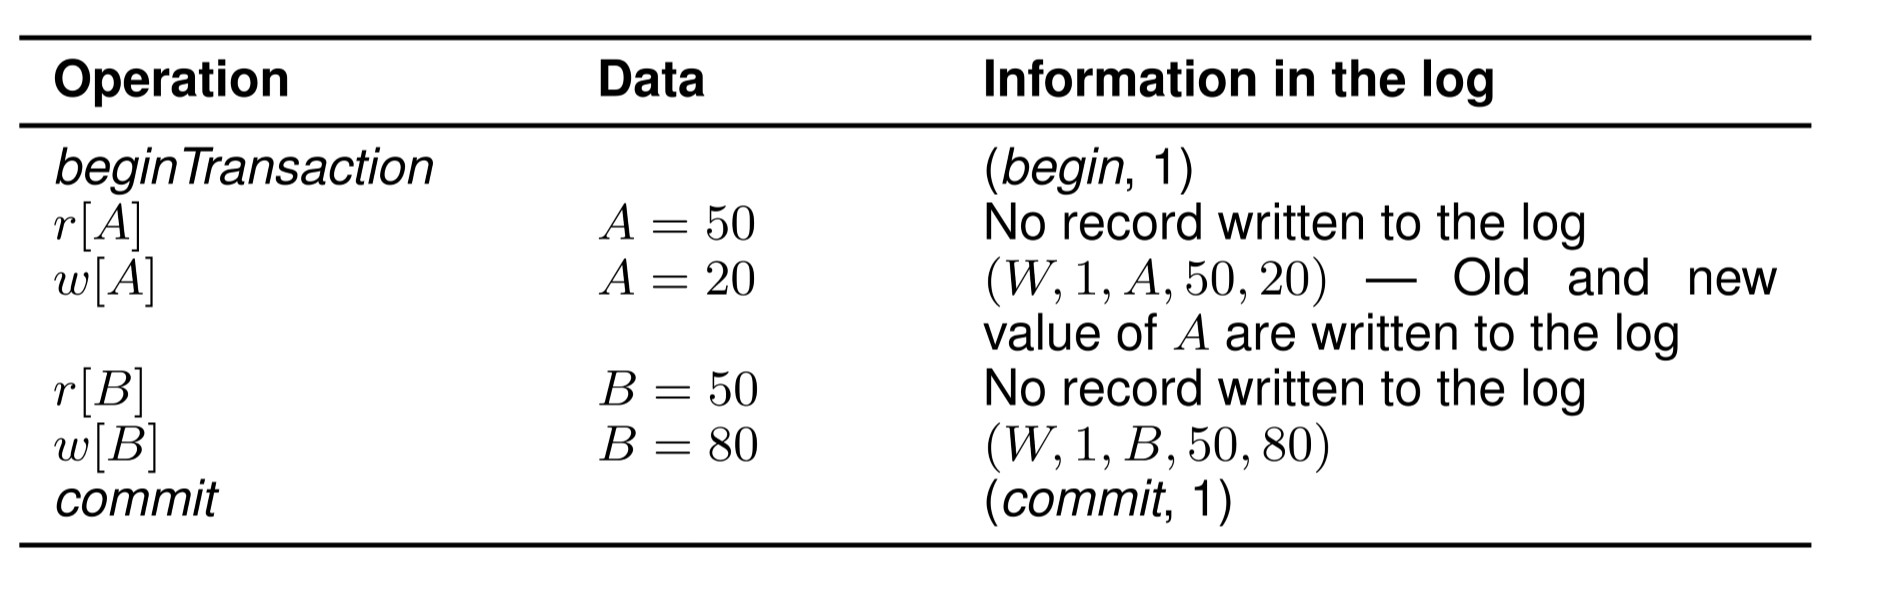
\includegraphics[scale = 0.6]{img/tr5.jpg}
		\label{tr2}
\end{figure}

\textbf{NOTE}:

\begin{itemize}

    \item the read operations do not affect the state of the database, and for this reason no record is written to the log;
    
    \item the exact content of the log depends on the algorithms of the transaction manager;
    
    \item in general a log is stored in a file buffered for efficiency reasons;
    
    \item we assume that the log is not buffered and each record is immediately written to the permanent memory
\end{itemize}

\subsubsection{Undo and Redo algorithms}
Recovery algorithms differ in the information they store in the log, in how they structure this information and, more importantly, in the time when the system transfers the pages updated by a transaction to the permanent memory. We say that a recovery algorithm requires an \textbf{undo} if an update of some uncommitted transaction is stored in the database. Should a transaction or a system failure occur, the recovery algorithm must undo the updates by copying the before-image of the page from the log to the database. 

\begin{figure}[h!]
		\centering
		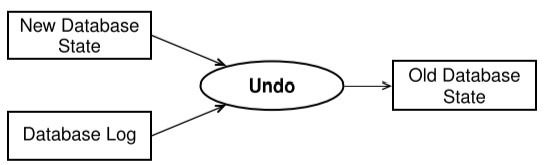
\includegraphics[scale = 1.3]{img/tr3.jpg}
		\label{tr2}
\end{figure}


We say that a recovery algorithm requires \textbf{redo} if a transaction is committed before all of its updates are stored in the database. Should a system failure occur after the transaction commits but before the updates are stored in the database, the recovery algorithm must redo the updates by copying the after-image of the page from the log to the database. 

\begin{figure}[H]
		\centering
		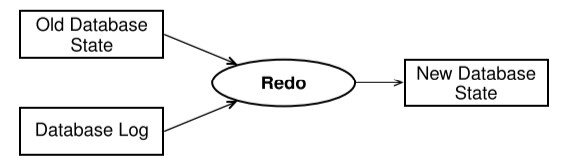
\includegraphics[scale = 1.3]{img/tr4.jpg}
		\label{tr2}
\end{figure}

A failure can happen also during the execution of a recovery procedure, and this requires the restart of the procedure. This means that for such procedures the \textit{idempotency} property must hold. That is, even if the operation is executed multiple times the effect is the same as if it is executed once. For the assumption that the entire page
is replaced, this property is automatically fulfilled.

\subsubsection{Checkpoint}
To reduce the work performed by a recovery procedure in the case of system failure, another information is written to the log, the so called \textbf{checkpoint} (CKP) event. There exists three methods of performing and recording checkpoints:

\begin{itemize}
    \item \textbf{commit-consistent checkpoint}:
    
    \begin{enumerate}
        \item the activation of new transactions is suspended 
        \item the systems waits for the completion of all active transactions
        \item all modified pages present in the buffer (dirty pages) are written to the permanent memory and the relevant records are written to the log. Here the permanent memory is forced so that all the transactions terminated before the checkpoint have their updates
        \item the CKP record is written to the log 
        \item a pointer to the CKP record is stored in a special file, called restart file.
        \item the system allows the activation of new transactions
        
    \end{enumerate}

    This strategy is simple but not efficient, because from (2) we derive that if we have long-time running transactions, we must wait a long time before the flushing of the dirty pages. This problem also affects the work that must be done in the case of restart. For this reason, we should perform this strategy when no transactions are running, but this condition is very demanding;

    \item \textbf{buffer-consistent checkpoint - Version 1}: in this case there's no waiting for active transactions termination, but the problem of the buffer flush operation (costly operation) is still present;

    \item \textbf{Fuzzy checkpoint (ARIES method)}

\end{itemize}

\subsection{Recovery algorithms}
The Recovery managers for the transactions management differ in the way they combine the undo and redo algorithms in order to recover the last consistent state of a DB. There are four possibilities: Undo-Redo, Undo-NoRedo, NoUndo-Redo, NoUndo-NoRedo. In the following sections we assume that a write in the log is forced to disk.

\subsubsection{Use of the Undo algorithm}
The use of the undo algorithm depends on the policy used to write pages updated by an active transactions to the DB:

\begin{itemize}

    \item \textit{deferred update} requires that updated pages cannot be written to the DB before the transaction has committed, and it is implemented by "pinning" the pages in the buffer until the end of the transaction. This policy is costly at the time of the commit, but it is more efficient from the point of view of the resource usage. An algorithm that adopts this policy is a \textit{NoUndo} type: when a system failure occurs, no undo is necessary since the DB has not been changed.

    \item \textit{immediate update} allows that updated pages can be written to the DB before the transaction has committed, and it is implemented by setting the page as "dirty" and by removing its pin. An algorithm that adopts this policy is a \textit{Undo} type: if a system failure occurs, the updates of the DB must be undone.
    
\end{itemize}

To \textbf{undo} the updates of a transaction, the following rule must be observed:

\begin{tcolorbox}[title = Undo rule (Write ahead log)]
    If a database page is updated before the transaction has committed, its before-image must have been previously written to the log file in the permanent memory.
\end{tcolorbox}

This rule allows an undo of a transaction in the case of abort by using the before-images from the log.

\subsubsection{Use of the Redo algorithm}

The use of the redo algorithm depends on the policy used to commit a transaction:

\begin{itemize}

    \item \textit{deferred commit} requires that all updated pages are written to the DB before the commit record has been written to the log. A transaction that implements this policy is a \textit{NoRedo} type: when a system failure occurs, no redo of the updates is necessary. A downside of this policy is that the buffer manager is forced to flush to the permanent memory all the updated pages before the commit operation;

    \item \textit{immediate commit} allows the commit record to be written to the log before all updated pages have been written to the DB. An algorithm that adopts this policy is a \textit{Redo} type, since it is necessary to redo all the updates in the case of a system failure. On the other hand, the buffer manager is free to flush the unpinned pages to the permanent memory when it considers appropriate.

\end{itemize}

To \textbf{redo} the updates of a transaction, the following rule must be observed:

\begin{tcolorbox}[title = Redo rule (commit rule)]
    Before a transaction can commit, the after-images produced by the transaction must have been written to the log file in the permanent memory.
\end{tcolorbox}

\subsubsection{No use of Undo and Redo algorithms}

\begin{itemize}
    \item NoUndo algorithm requires that all the updates of a transaction must be in the database after the transaction has committed;
    \item NoRedo algorithm requires that all the updates of a transaction must be in the database before the transaction has committed
\end{itemize}

Therefore:

\begin{tcolorbox}
     A \textbf{NoUndo-NoRedo} algorithm requires that all the updates of a transaction must be in the database neither before nor after the transaction has committed.
\end{tcolorbox}

This condition is preserved if the commit operation atomically writes all the updates of a transaction to the DB and mark the transactions as committed: this is feasible using the \textbf{shadow pages}. 

The implementation of the shadow pages is based on the \textit{Page table}, a permanent memory index that maps each page identifier to the physical address where the page is stored. Moreover, there is the \textit{descriptor}, which is a record that contains a pointer to the Page table.

\begin{figure}[h!]
		\centering
		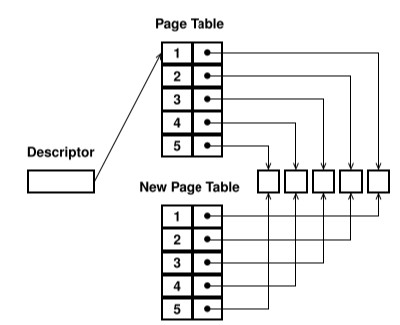
\includegraphics[scale = 1.3]{img/tr6.jpg}
		\label{tr2}
\end{figure}

When a transaction starts, a copy of the Page table is created in the permanent memory (\textit{New page table}), and it is used by the transaction. When a transaction updates for the first time a page: 

\begin{enumerate}
    \item a new database page is created, the \textit{current} page with a certain address $p$, whereas the old page becomes a \textit{shadow page}
    
    \item the New Page Table is updated so that the first element contains the physical address $p$ of the \textit{current page}
\end{enumerate}

\begin{figure}[h!]
		\centering
		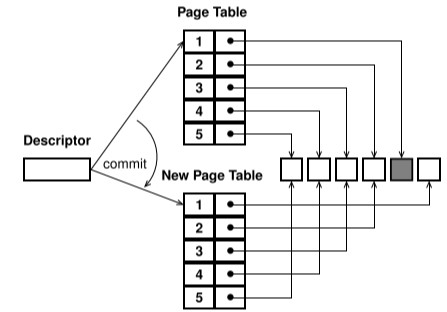
\includegraphics[scale = 1.3]{img/tr7.jpg}
		\label{tr2}
\end{figure}


When the transaction reaches the commit point, the system should substitute all the shadow pages with an atomic action, otherwise if a failure happen the database would be left in an incorrect state. This atomic action is implemented by executing the following steps:

\begin{enumerate}
    \item the pages updated in the buffer are written to the permanent memory
    \item the descriptor of the database is updated with an atomic operation
\end{enumerate}

\textbf{NOTE}: 

\begin{itemize}

    \item no need for undo/redo, but this technique is difficult to be applied if the system manages concurrent transactions;
    
    \item if the number of abortion/rollbacks is not high, the undo-redo policy is the preferred one, since it is more efficient.
    
\end{itemize}

\subsection{Recovery from system and media failure}

In the case of \textbf{system failures}, in order to recover the database, the \textit{restart} operator is invoked to perform the following steps (\textit{warm restart}):

\begin{itemize}
    \item bring the database in its committed state with respect to the execution up to the to the system failure;
    \item restart the normal system operations.
\end{itemize}

And is described with two phases: 

\begin{itemize}

    \item in the \textbf{rollback} phase the log is read from the end to the beginning:
    
    \begin{itemize}
    
        \item to undo, if necessary, the updates of the non terminated transactions;
        
        \item to find the set of the identifiers of the transactions which are terminated successfully in order to redo their operations.
        
    \end{itemize}

    \item in the \textbf{rollforward} phase the log is read onward from the first record after the checkpoint to redo all the operations of the terminated transaction
    
\end{itemize}

In this example, both $T_3$ and $T_5$ must be undone, while $T_2$ and $T_4$ must be redone.

\begin{figure}[h!]
		\centering
		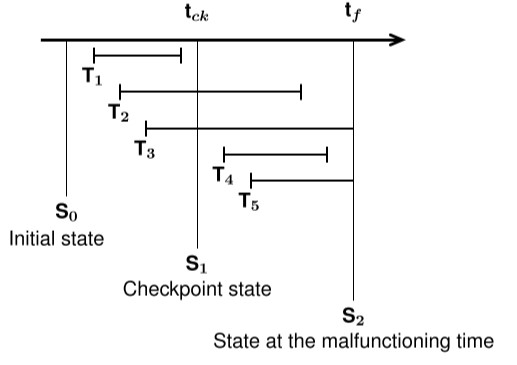
\includegraphics[scale = 1.3]{img/tr8.jpg}
		\label{tr2}
\end{figure}

Picture \ref{tr9} and \ref{tr10} show the actions to be performed in the \textit{rollback} and \textit{rollforward} phases of the restart procedure: $L_r$ indicates the set of transactions to be redone, while $L_u$ indicates the set of transactions to be undone.

\begin{figure}[h!]
		\centering
		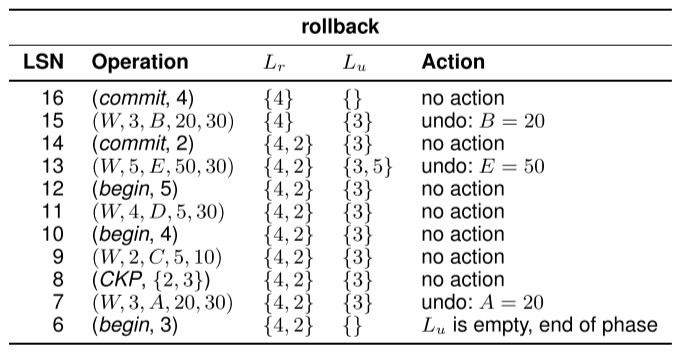
\includegraphics[scale = 1.3]{img/tr9.jpg}
		\label{tr9}
\end{figure}

\begin{figure}[h!]
		\centering
		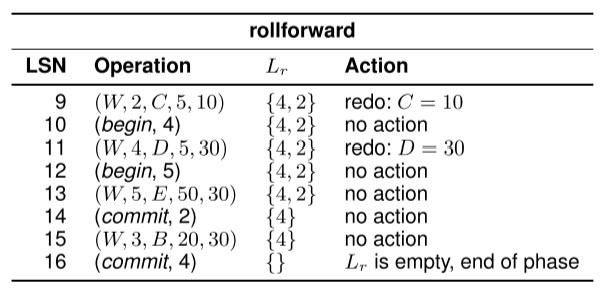
\includegraphics[scale = 1.3]{img/tr10.jpg}
		\label{tr10}
\end{figure}

In the case of \textbf{media failure}, a \textit{cold restart} is performed through the following steps:

\begin{itemize}
    \item the most recent database backup is reloaded;
    \item a \textit{rollback} phase is performed on the log;
    \item a \textit{rollforward} phase is performed to update the copy of the database
\end{itemize}

